
\begin{frame}
 \frametitle{Классификация}
 \begin{itemize}
   \item Архитектура набора команд (Instruction set architecture)
   \item Микроархитектура
 \end{itemize}
\end{frame}
\subsection{Mикроархитектура}
\begin{frame}
 \frametitle{Микроархитектура}
 \textbf{Микроархитектура} -- определяет конкретную реализацию системы команд в железе. 

 \textbf{Важные элементы}
 \begin{itemize}
  \item Количество тактов на инструкцию
  \item Длина и структура конвейера
  \item Размер и структура кэшей
  \item Организация периферийных шин
 \end{itemize}
\end{frame}

\begin{frame}
  \frametitle{Пример: микроархитектура Intel Core}
  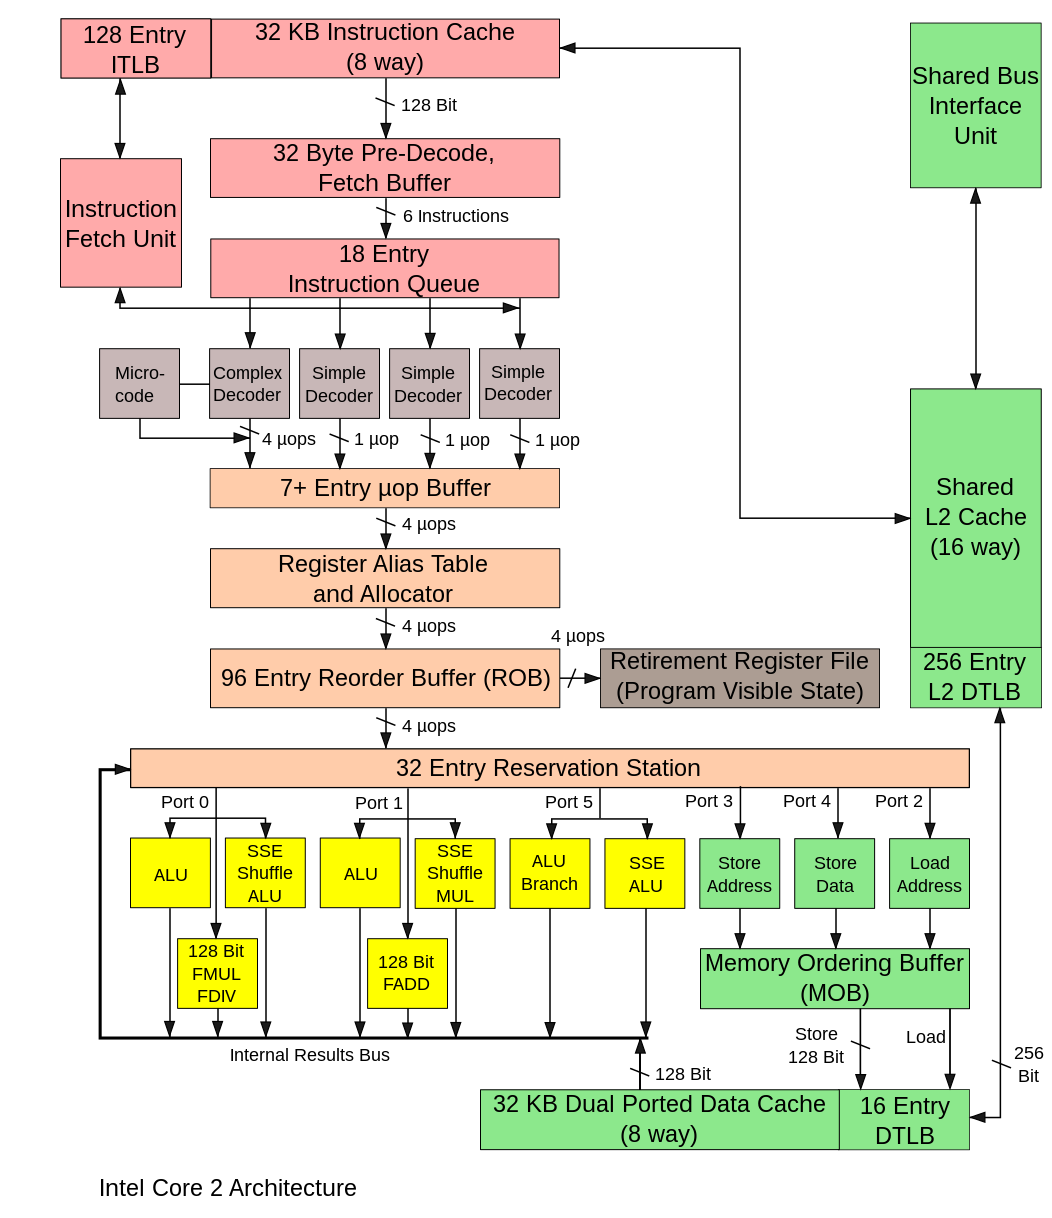
\includegraphics[height=6cm]{slides/processor_arch/Intel_Core2_arch.png}
\end{frame}
\subsection{Архитектура системы команд}
\begin{frame}
 \frametitle{Архитектура системы команд}
 \begin{center}
   {\bf\large Основные возможности}
 \end{center}
 \begin{itemize}
     \item Гарвардская/фон Неймановская
     \item RISC/CISC/VLIW/EPIC
     \item Разрядность (8/16/32/64)
     \item Число и типы регистров
     \item Максимальное число операндов (1,2,3,\dots) 
     \item Тип операндов (Регистр-регистр, Регистр-память, Память-память, Стековая машина)
     \item Кодировка инструкций (переменной длины, постоянной длины)
     \item Порядок байтов (старшего к младшему (big endian), младшего к старшему (little endian))
     \item Расширения
 \end{itemize}
\end{frame}

\begin{frame}
  \frametitle{Intel x86}
  \begin{itemize}
    \item фон Неймановская (модифицированная)
    \item CISC
    \item 16-64 бита 
    \item 8 специализированных регистров, 3-6 сегментных регистров, IP, 8 неспециализированных регистров, SIMD
    \item Max operands 2(3 for AVX)
    \item Регистр-память
    \item Переменной длины
    \item Little endian
    \item SSE, MMX, 3dNow
  \end{itemize}
\end{frame}

\begin{frame}
  \frametitle{ARM/ARMv7}
  \begin{itemize}
      \item фон Неймановская модифицированная
      \item RISC
      \item 16/32
      \item 7/15 неспециализированных регистров
      \item Регистр-регистр
      \item Фиксированная (32/16), Thumb-2 переменной длины
      \item Little/Big endian (mostly little)
      \item VFP, NEON, Jazelle,TrustZone
  \end{itemize}
\end{frame}

\begin{frame}
  \frametitle{MIPS}
  \begin{itemize}
      \item фон Неймановская модифицированая
      \item RISC
      \item 32/64
      \item 4-32 неспециализированных регистра
      \item Регистр-регистр
      \item Фиксированная(32)
      \item Big/Little endian
      \item MDMX, MIPS-3d
      \item задержка перехода (branch delay slot)
   \end{itemize}
\end{frame}
\subsection{Виртуальная адресация}
\begin{frame}
  \frametitle{Виртуальное адресное пространство}
  \begin{center}
    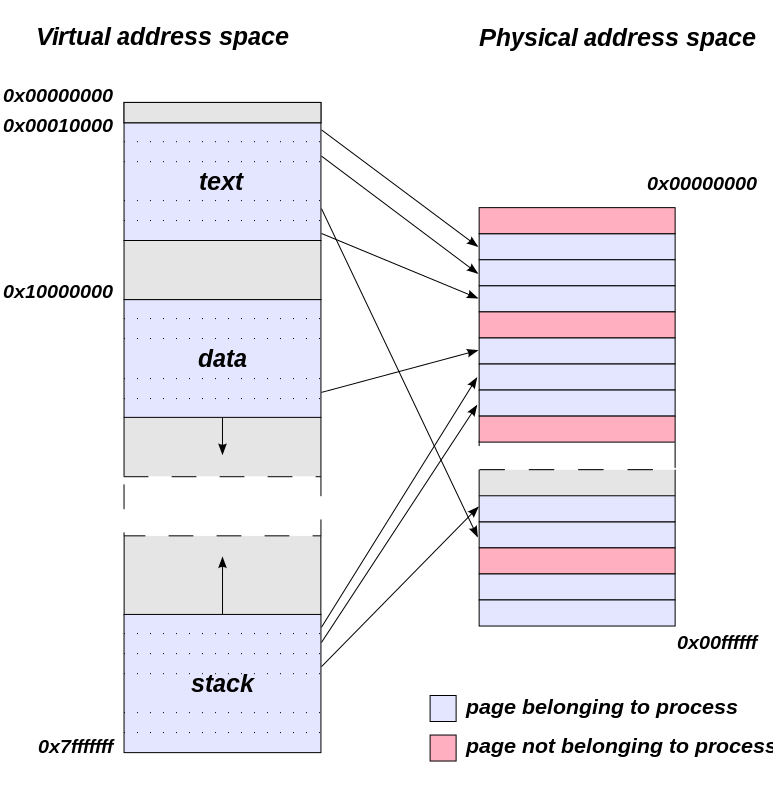
\includegraphics[height=6cm]{slides/processor_arch/Virtual_address_space_and_physical_address_space_relationship.png}
  \end{center}
\end{frame}
\begin{frame}
  \frametitle{Таблица страниц(page table):Intel PAE}
  \begin{center}
    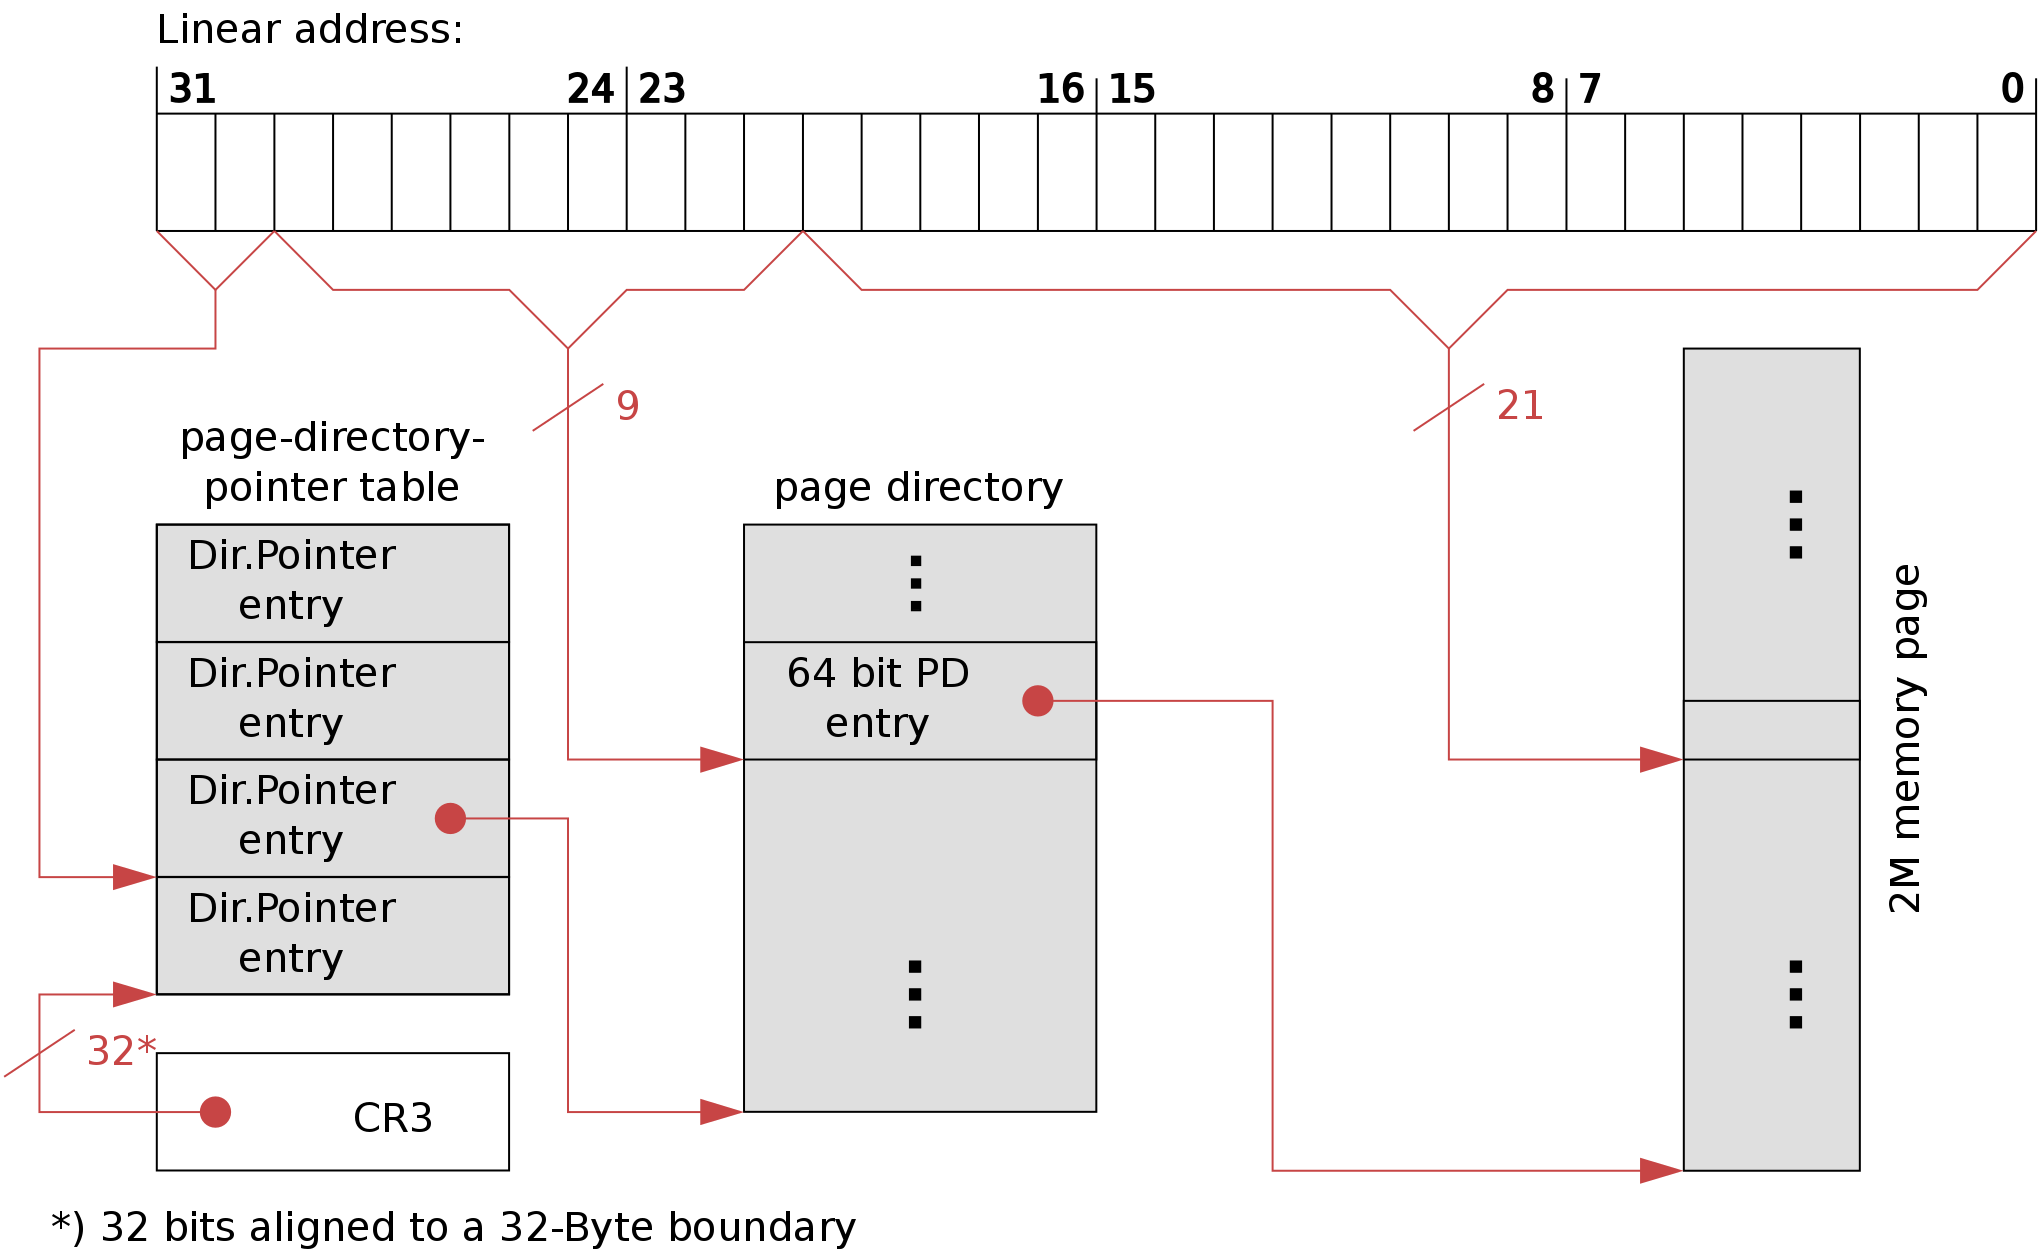
\includegraphics[height=6cm]{slides/processor_arch/X86_Paging_PAE_2M.png}
  \end{center}
\end{frame}

\begin{frame}
  \frametitle{Таблица страниц: ARM}
  \begin{center}
    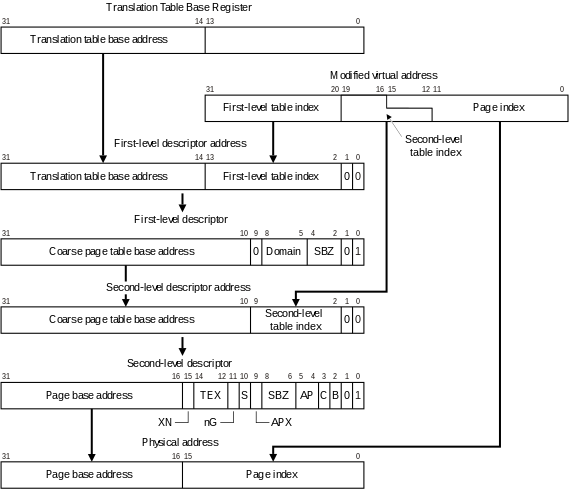
\includegraphics[height=6cm]{slides/processor_arch/large_page_table_walk_armv6_format.png}
  \end{center}
\end{frame}

\begin{frame}
  \frametitle{Буфер ассоциативной трансляции(TLB)}
  \begin{center}
    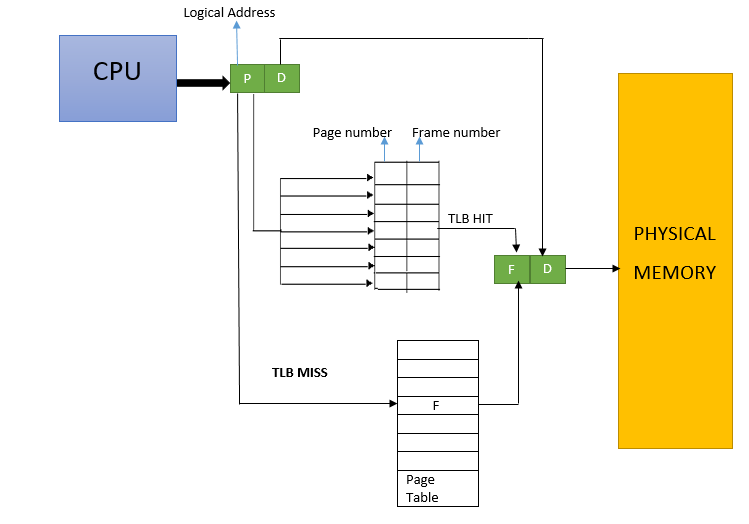
\includegraphics[height=6cm]{slides/processor_arch/Translation_Lookaside_Buffer.png}
  \end{center}
\end{frame}

